\documentclass[ignorenonframetext,]{beamer}
\setbeamertemplate{caption}[numbered]
\setbeamertemplate{caption label separator}{: }
\setbeamercolor{caption name}{fg=normal text.fg}
\beamertemplatenavigationsymbolsempty
\usepackage{lmodern}
\usepackage{amssymb,amsmath}
\usepackage{ifxetex,ifluatex}
\usepackage{fixltx2e} % provides \textsubscript
\ifnum 0\ifxetex 1\fi\ifluatex 1\fi=0 % if pdftex
  \usepackage[T1]{fontenc}
  \usepackage[utf8]{inputenc}
\else % if luatex or xelatex
  \ifxetex
    \usepackage{mathspec}
  \else
    \usepackage{fontspec}
  \fi
  \defaultfontfeatures{Ligatures=TeX,Scale=MatchLowercase}
\fi
% use upquote if available, for straight quotes in verbatim environments
\IfFileExists{upquote.sty}{\usepackage{upquote}}{}
% use microtype if available
\IfFileExists{microtype.sty}{%
\usepackage{microtype}
\UseMicrotypeSet[protrusion]{basicmath} % disable protrusion for tt fonts
}{}
\newif\ifbibliography
\hypersetup{
            pdftitle={CO2 emissions for Ulm for 1-2 FH buildings},
            pdfauthor={Bhaskar Kamble},
            pdfborder={0 0 0},
            breaklinks=true}
\urlstyle{same}  % don't use monospace font for urls
\usepackage{graphicx,grffile}
\makeatletter
\def\maxwidth{\ifdim\Gin@nat@width>\linewidth\linewidth\else\Gin@nat@width\fi}
\def\maxheight{\ifdim\Gin@nat@height>\textheight0.8\textheight\else\Gin@nat@height\fi}
\makeatother
% Scale images if necessary, so that they will not overflow the page
% margins by default, and it is still possible to overwrite the defaults
% using explicit options in \includegraphics[width, height, ...]{}
\setkeys{Gin}{width=\maxwidth,height=\maxheight,keepaspectratio}

% Prevent slide breaks in the middle of a paragraph:
\widowpenalties 1 10000
\raggedbottom

\AtBeginPart{
  \let\insertpartnumber\relax
  \let\partname\relax
  \frame{\partpage}
}
\AtBeginSection{
  \ifbibliography
  \else
    \let\insertsectionnumber\relax
    \let\sectionname\relax
    \frame{\sectionpage}
  \fi
}
\AtBeginSubsection{
  \let\insertsubsectionnumber\relax
  \let\subsectionname\relax
  \frame{\subsectionpage}
}

\setlength{\parindent}{0pt}
\setlength{\parskip}{6pt plus 2pt minus 1pt}
\setlength{\emergencystretch}{3em}  % prevent overfull lines
\providecommand{\tightlist}{%
  \setlength{\itemsep}{0pt}\setlength{\parskip}{0pt}}
\setcounter{secnumdepth}{0}

\title{CO2 emissions for Ulm for 1-2 FH buildings}
\author{Bhaskar Kamble}
\date{4 März 2019}

\begin{document}
\frame{\titlepage}

\begin{frame}{Introduction}

CO2 emissions for Ulm\ldots{}

\end{frame}

\begin{frame}{Ulm, 1-2 FH}

This time I replace the 2018 value by the trend value.

\end{frame}

\begin{frame}{Verbrauchsanteile nach Energieträger - data}

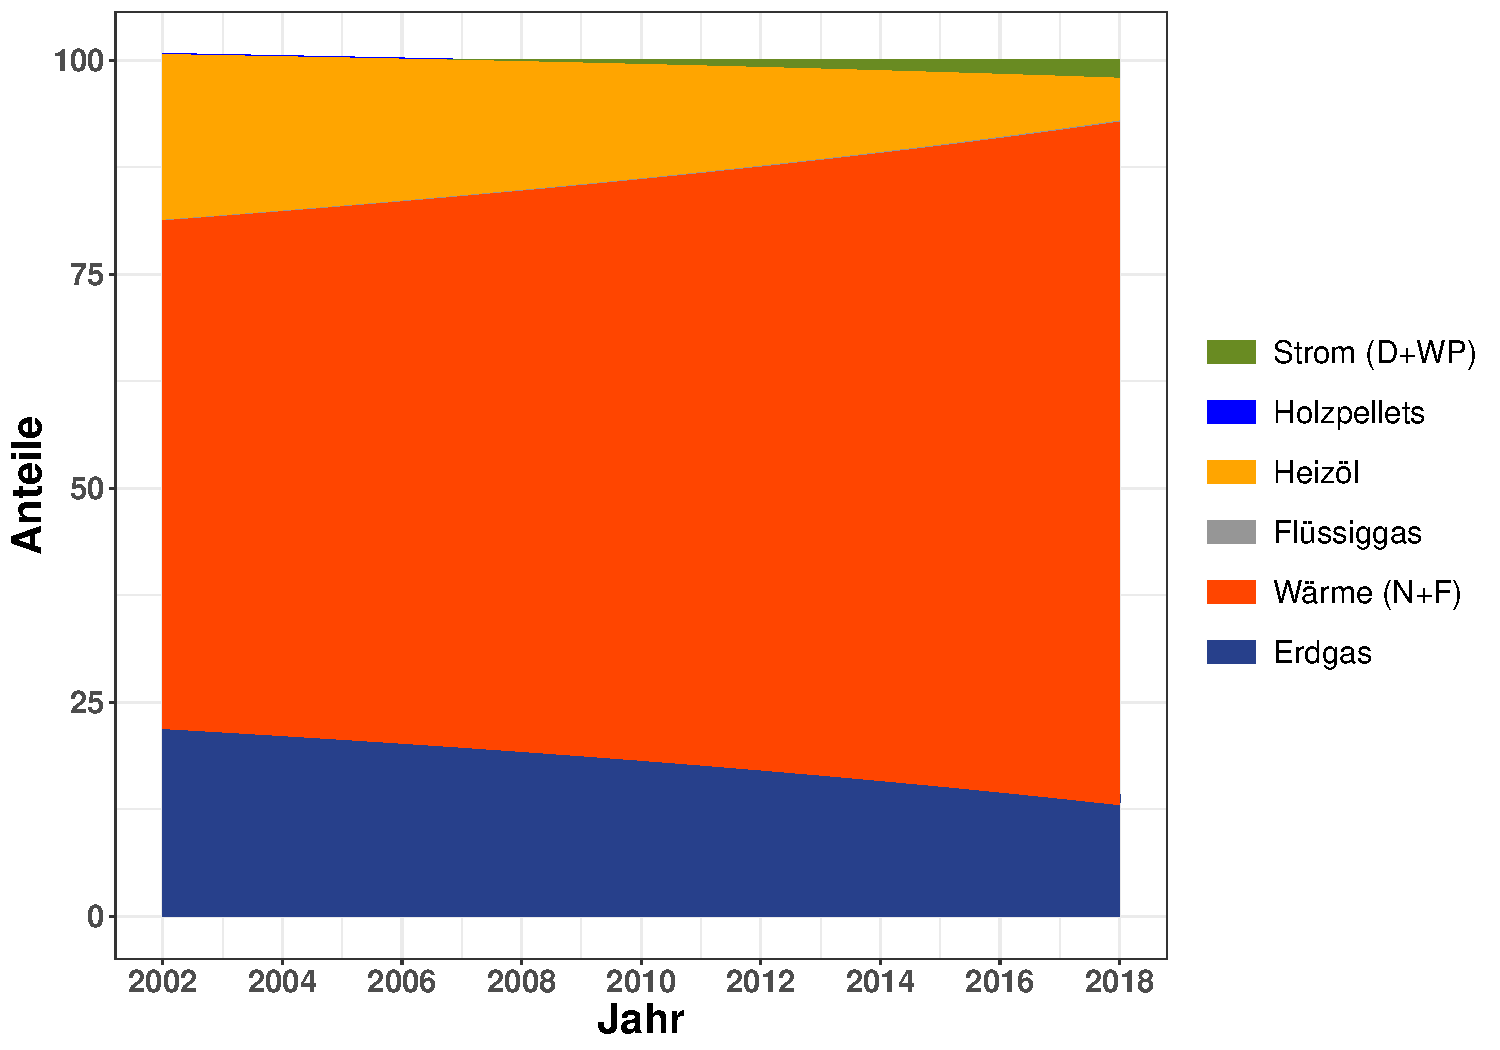
\includegraphics{UlmPresentationCO2BalanceSFH_v3_files/figure-beamer/unnamed-chunk-10-1.pdf}

\end{frame}

\begin{frame}{Verbrauchsanteile nach Energieträger - graph}

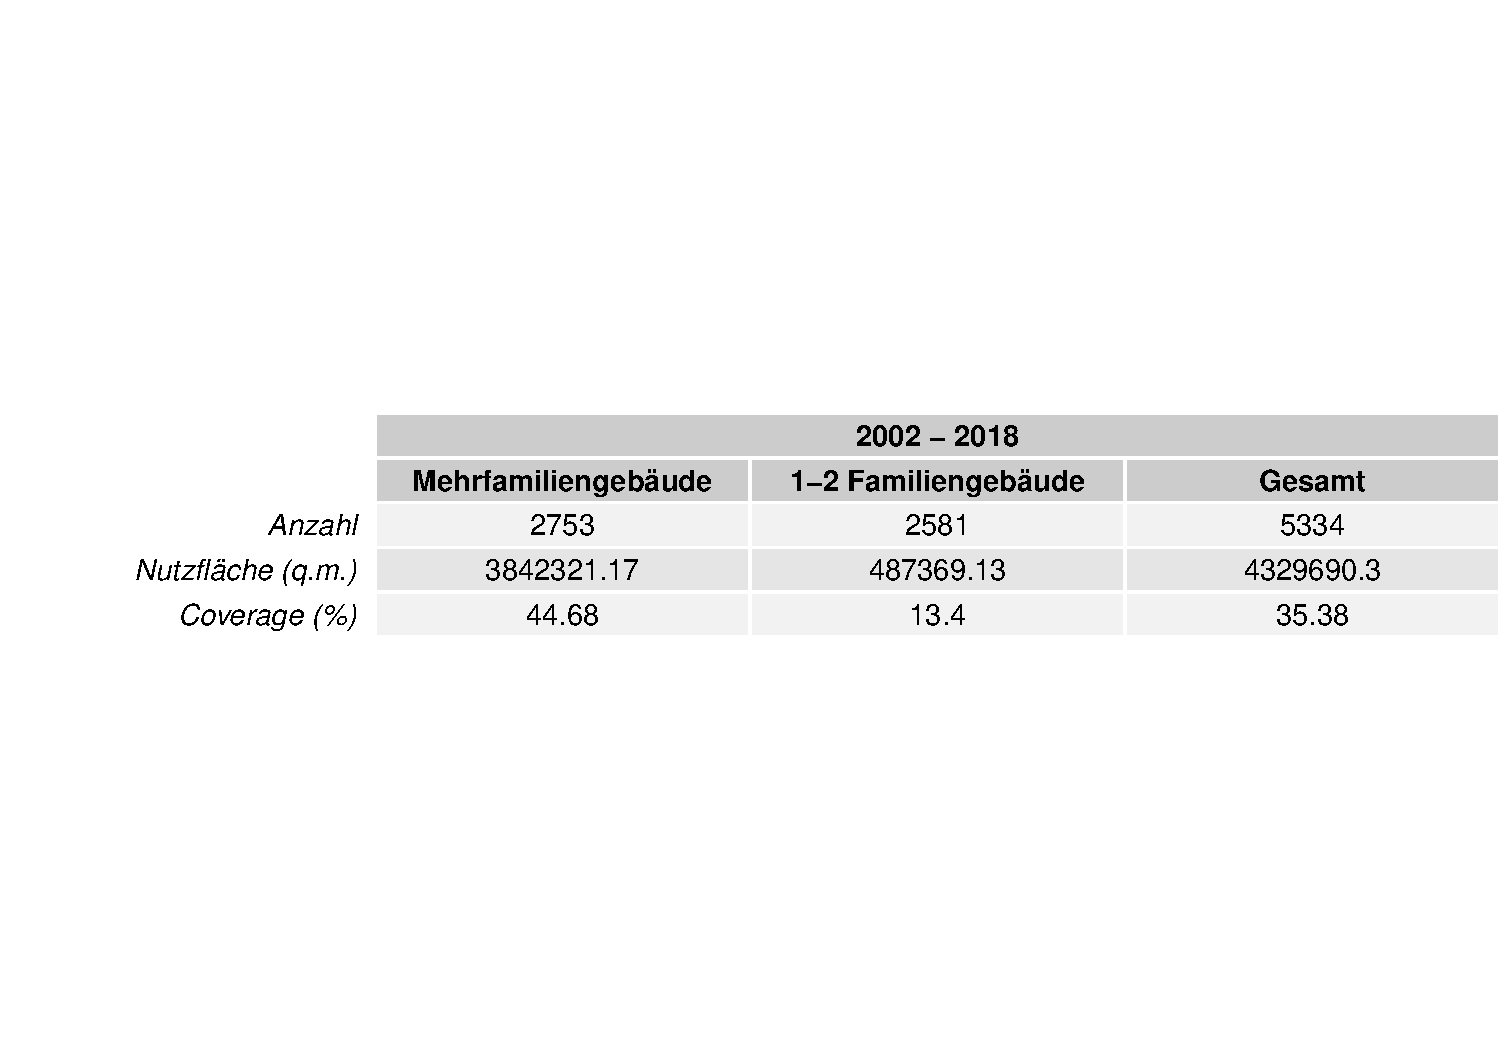
\includegraphics{UlmPresentationCO2BalanceSFH_v3_files/figure-beamer/unnamed-chunk-16-1.pdf}

\end{frame}

\begin{frame}{Verbrauchsanteile nach Energieträger - linear graph}

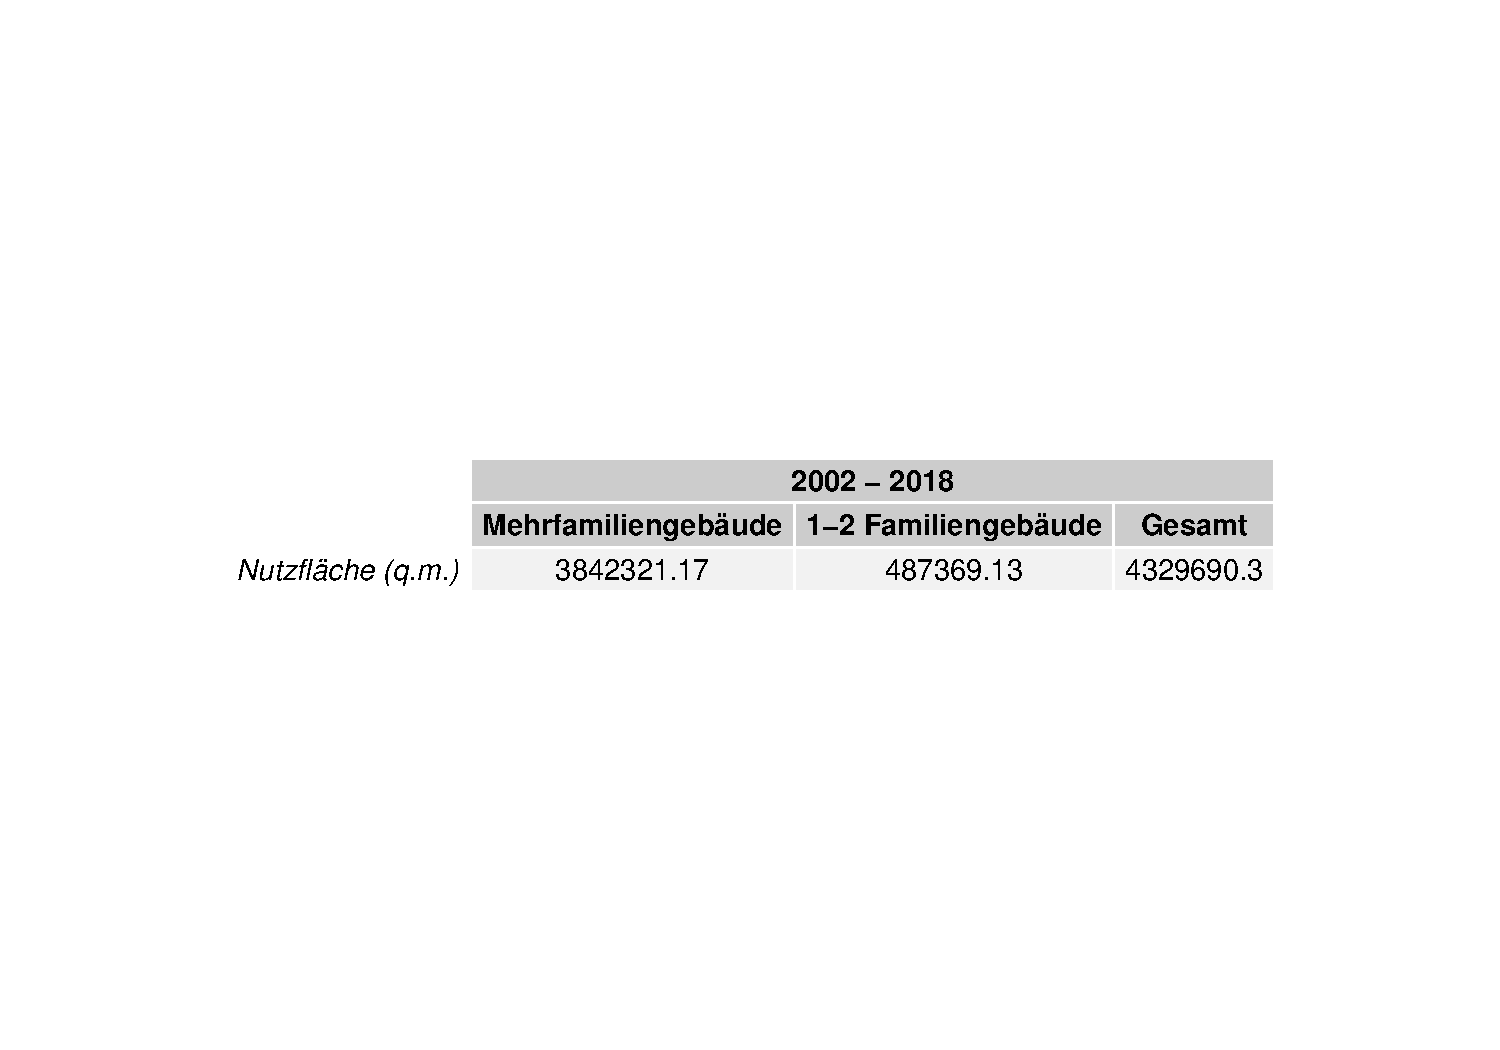
\includegraphics{UlmPresentationCO2BalanceSFH_v3_files/figure-beamer/unnamed-chunk-17-1.pdf}

\end{frame}

\begin{frame}{Flächeanteile nach Energieträger - data}

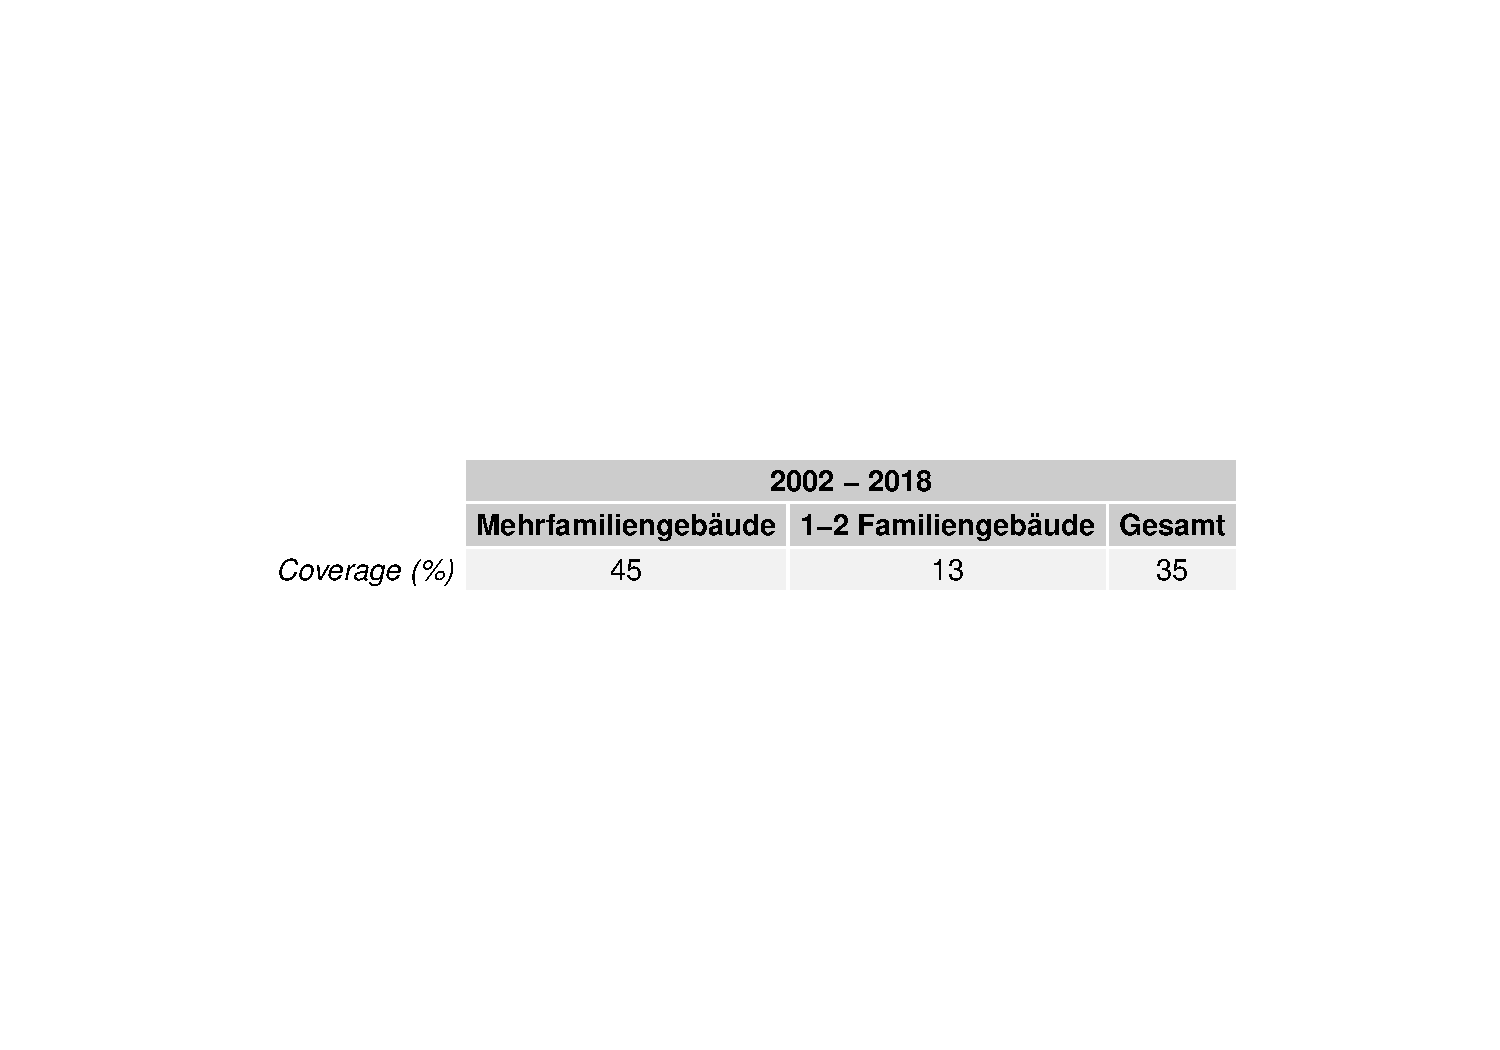
\includegraphics{UlmPresentationCO2BalanceSFH_v3_files/figure-beamer/unnamed-chunk-20-1.pdf}

\end{frame}

\begin{frame}{Flächeanteile nach Energieträger - graph}

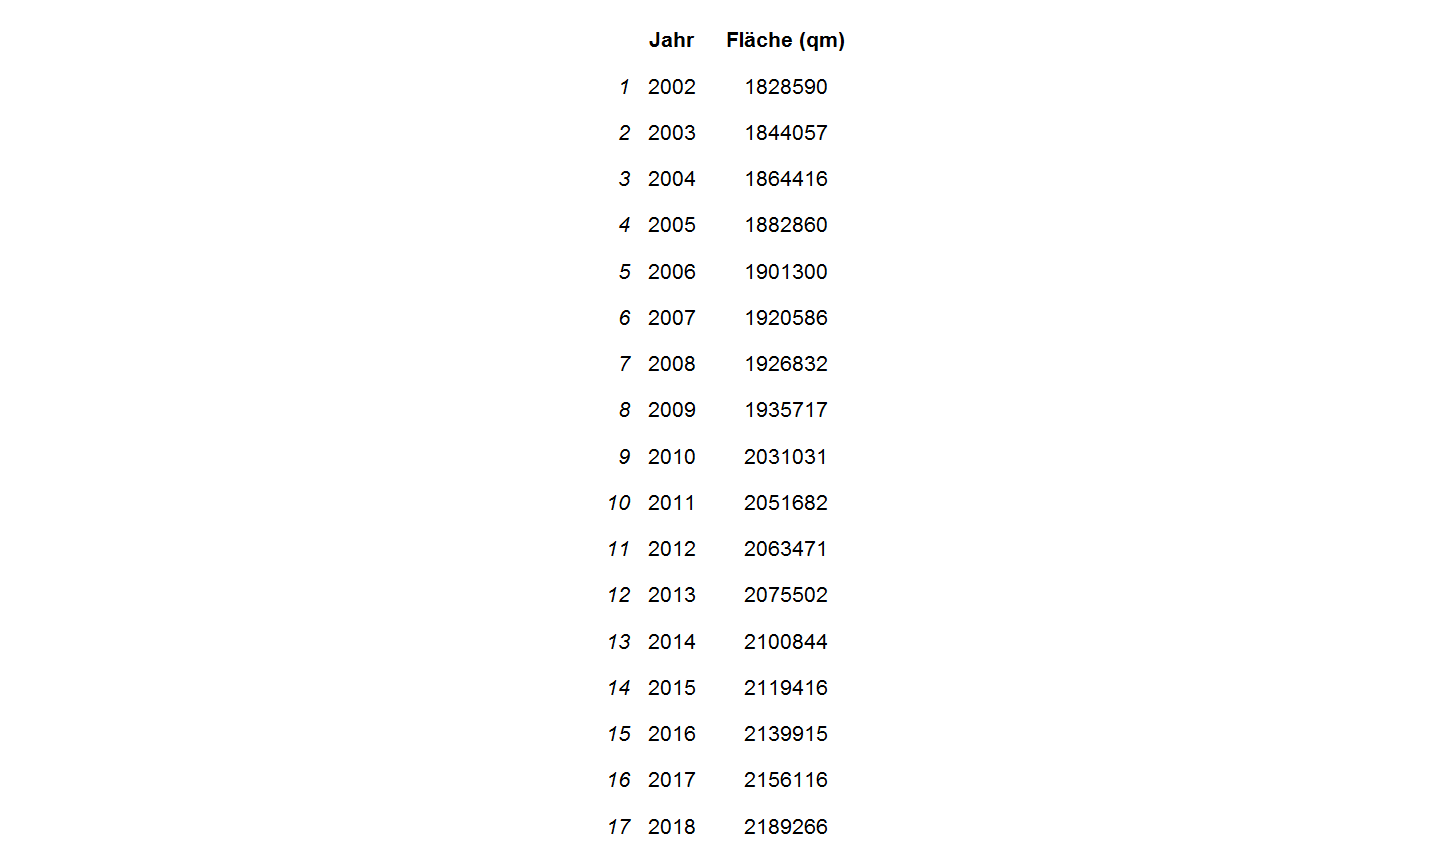
\includegraphics{UlmPresentationCO2BalanceSFH_v3_files/figure-beamer/unnamed-chunk-22-1.pdf}

\end{frame}

\begin{frame}{Flächeanteile nach Energieträger - linear graph}

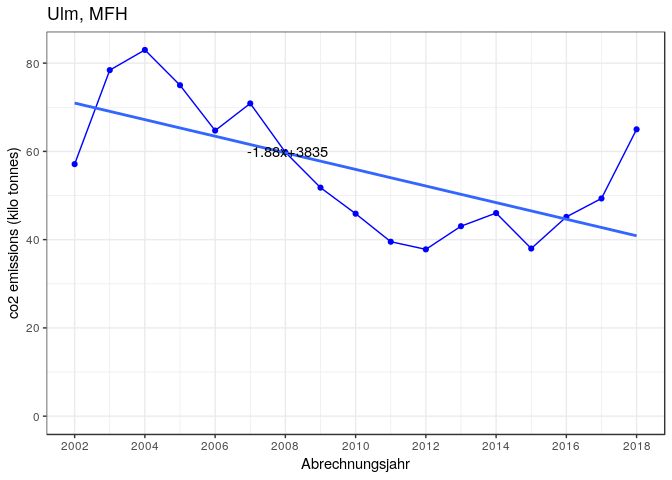
\includegraphics{UlmPresentationCO2BalanceSFH_v3_files/figure-beamer/unnamed-chunk-24-1.pdf}

\end{frame}

\begin{frame}{Total heated area - official figures}

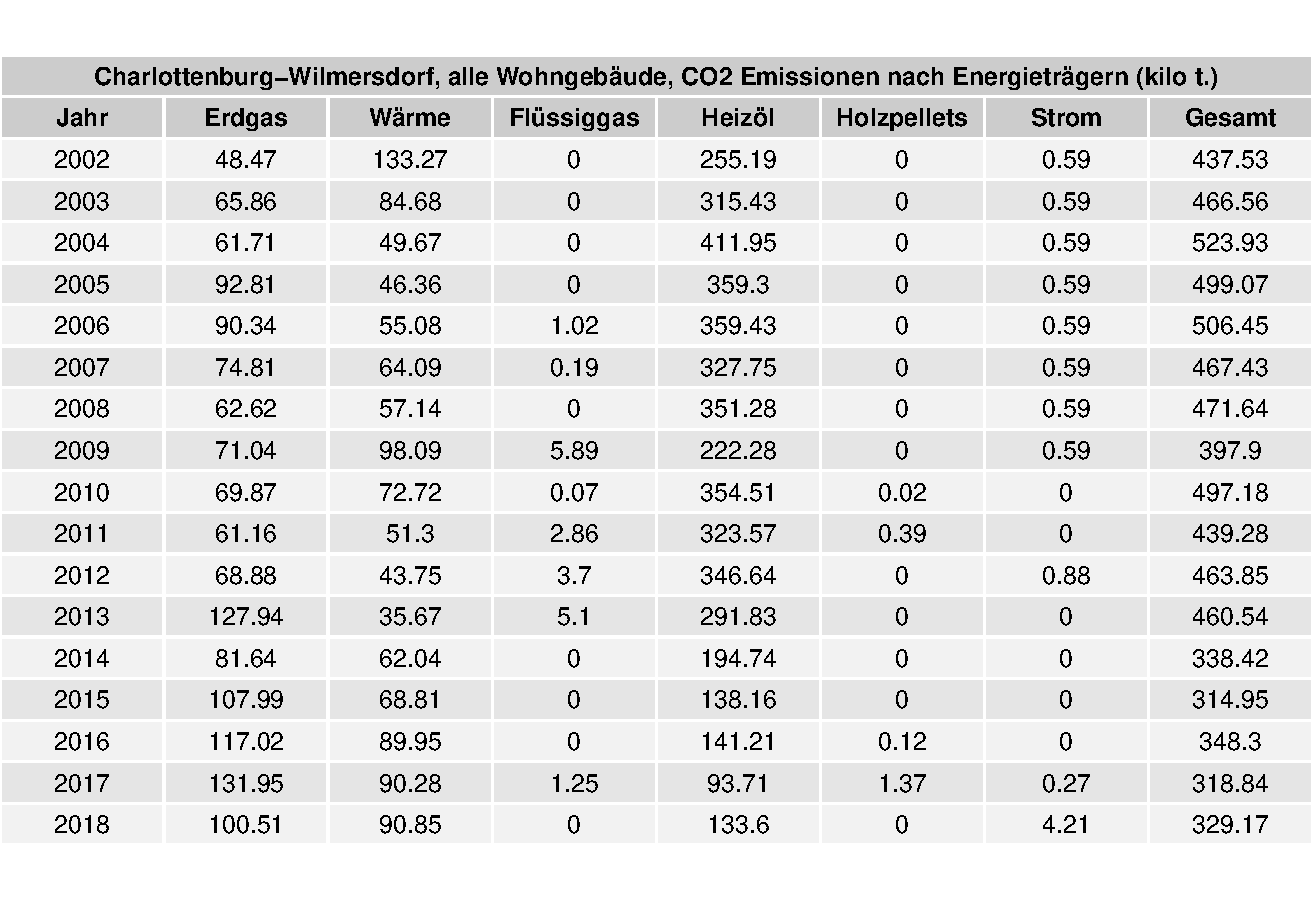
\includegraphics{UlmPresentationCO2BalanceSFH_v3_files/figure-beamer/unnamed-chunk-25-1.pdf}

\end{frame}

\begin{frame}{Fläche nach Energietraeger - data}

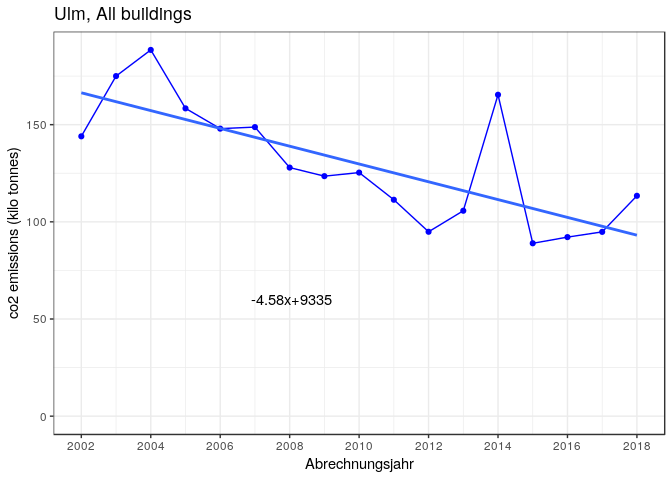
\includegraphics{UlmPresentationCO2BalanceSFH_v3_files/figure-beamer/unnamed-chunk-26-1.pdf}

\end{frame}

\begin{frame}{Fläche nach Energietraeger - graph}

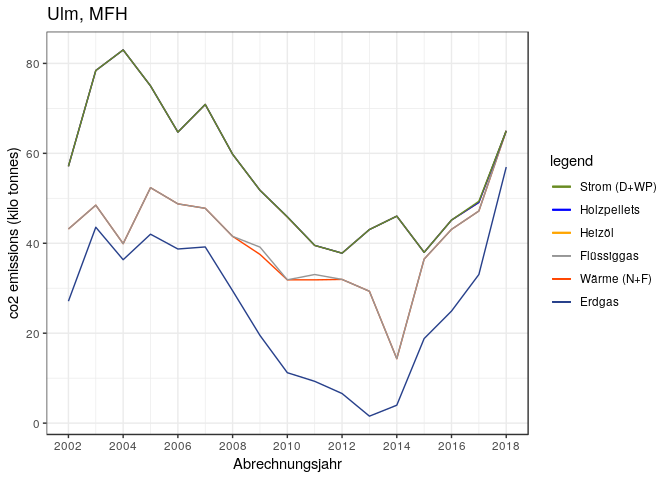
\includegraphics{UlmPresentationCO2BalanceSFH_v3_files/figure-beamer/unnamed-chunk-28-1.pdf}

\end{frame}

\begin{frame}{Fläche nach Energietraeger - linear graph}

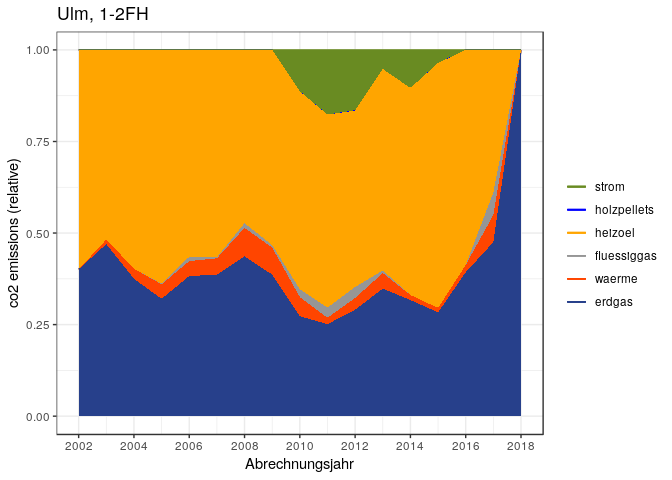
\includegraphics{UlmPresentationCO2BalanceSFH_v3_files/figure-beamer/unnamed-chunk-30-1.pdf}

\end{frame}

\begin{frame}{Verbrauch nach Energieträgers - data}

\includegraphics{UlmPresentationCO2BalanceSFH_v3_files/figure-beamer/unnamed-chunk-32-1.pdf}

\end{frame}

\begin{frame}{Verbrauch nach Energieträgers - graph}

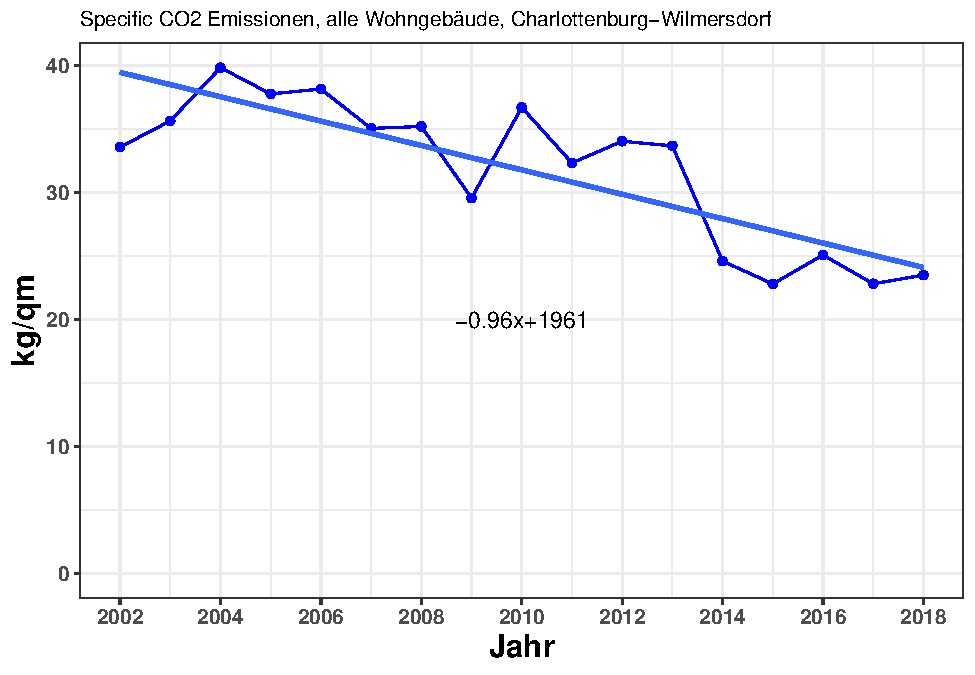
\includegraphics{UlmPresentationCO2BalanceSFH_v3_files/figure-beamer/unnamed-chunk-34-1.pdf}

\end{frame}

\begin{frame}{Verbrauch nach Energieträgers - linear graph}

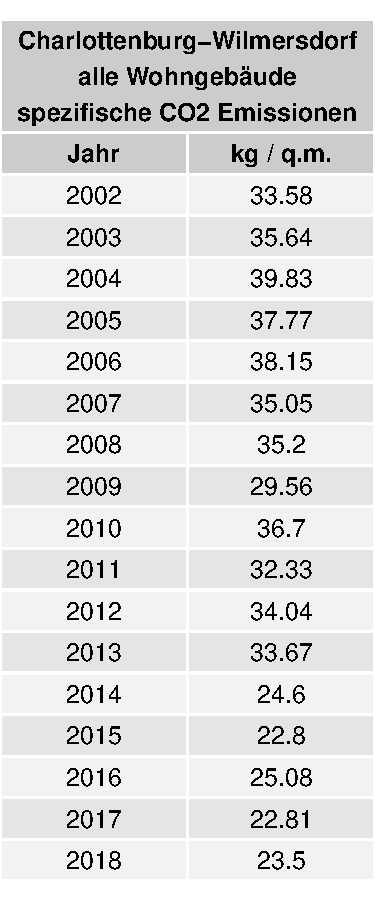
\includegraphics{UlmPresentationCO2BalanceSFH_v3_files/figure-beamer/unnamed-chunk-36-1.pdf}

\end{frame}

\begin{frame}{Verbrauchsanteile nach Energieträgers - data}

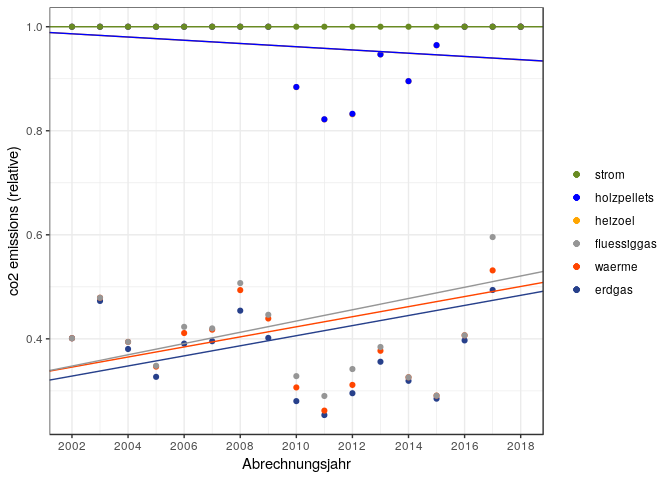
\includegraphics{UlmPresentationCO2BalanceSFH_v3_files/figure-beamer/unnamed-chunk-38-1.pdf}

\end{frame}

\begin{frame}{Verbrauchsanteile nach Energieträgers - graph}

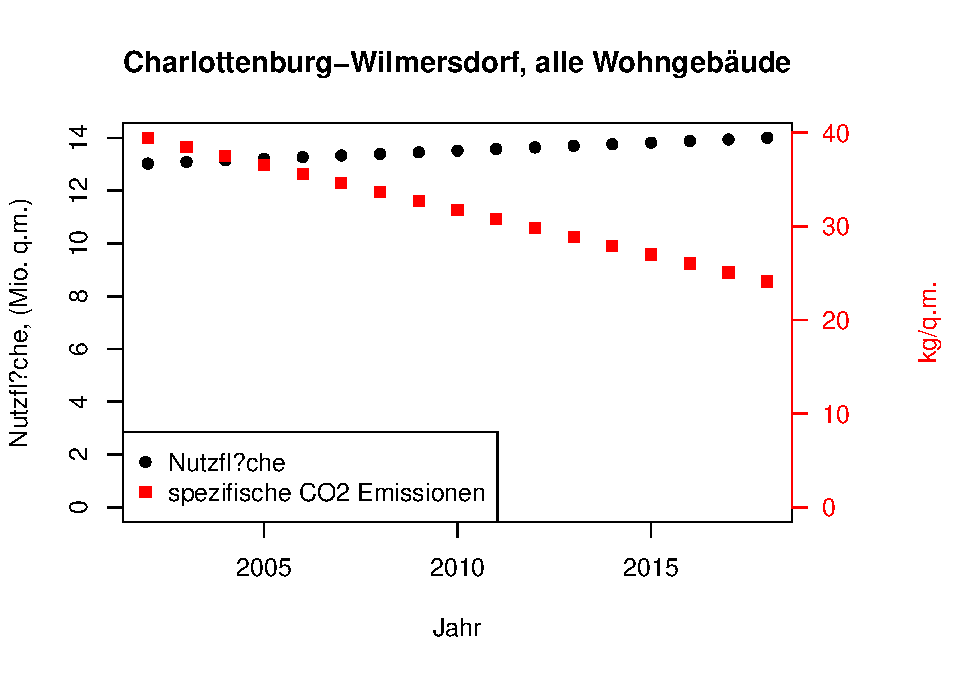
\includegraphics{UlmPresentationCO2BalanceSFH_v3_files/figure-beamer/unnamed-chunk-40-1.pdf}

\end{frame}

\begin{frame}{CO2 coefficients}

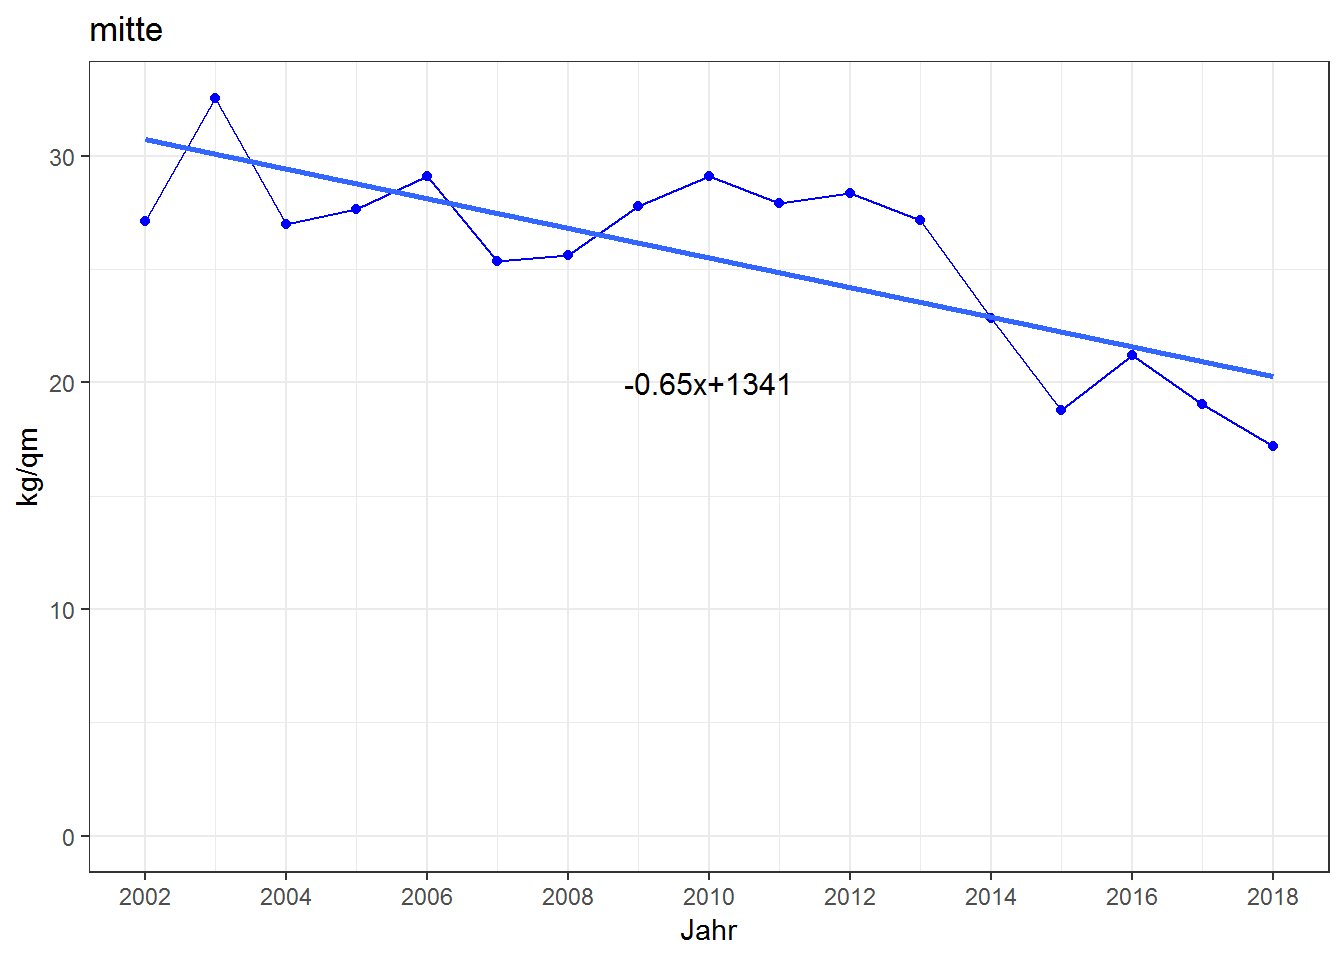
\includegraphics{UlmPresentationCO2BalanceSFH_v3_files/figure-beamer/unnamed-chunk-41-1.pdf}

\end{frame}

\begin{frame}{CO2 emissions by energieträger - data}

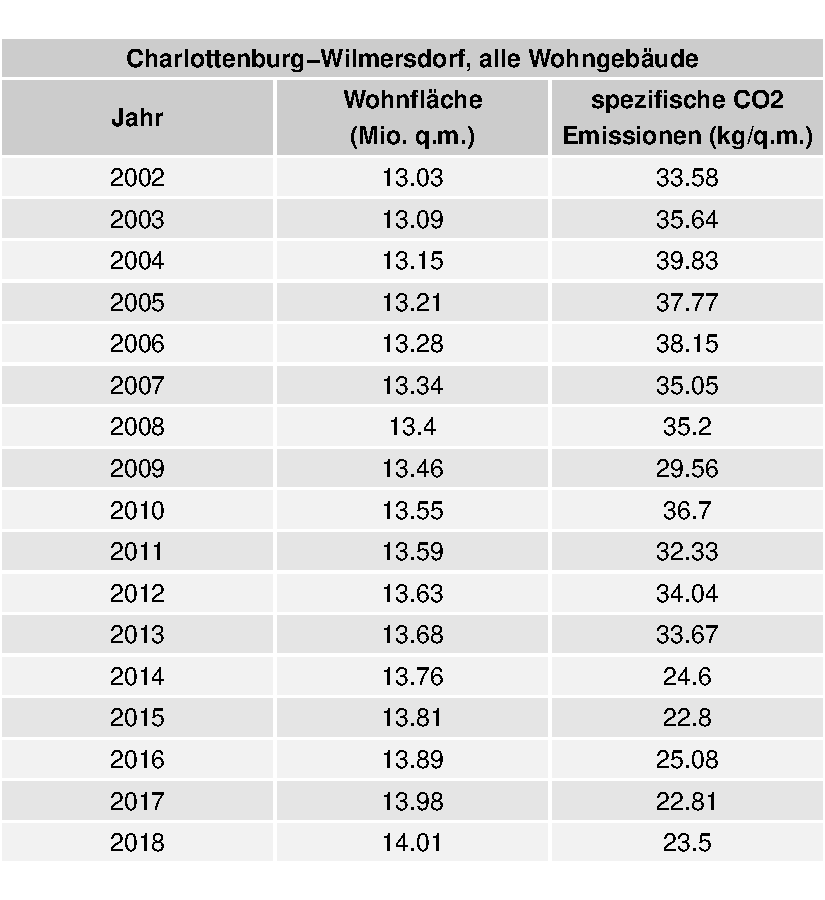
\includegraphics{UlmPresentationCO2BalanceSFH_v3_files/figure-beamer/unnamed-chunk-42-1.pdf}

\end{frame}

\begin{frame}{CO2 emissions - total graph}

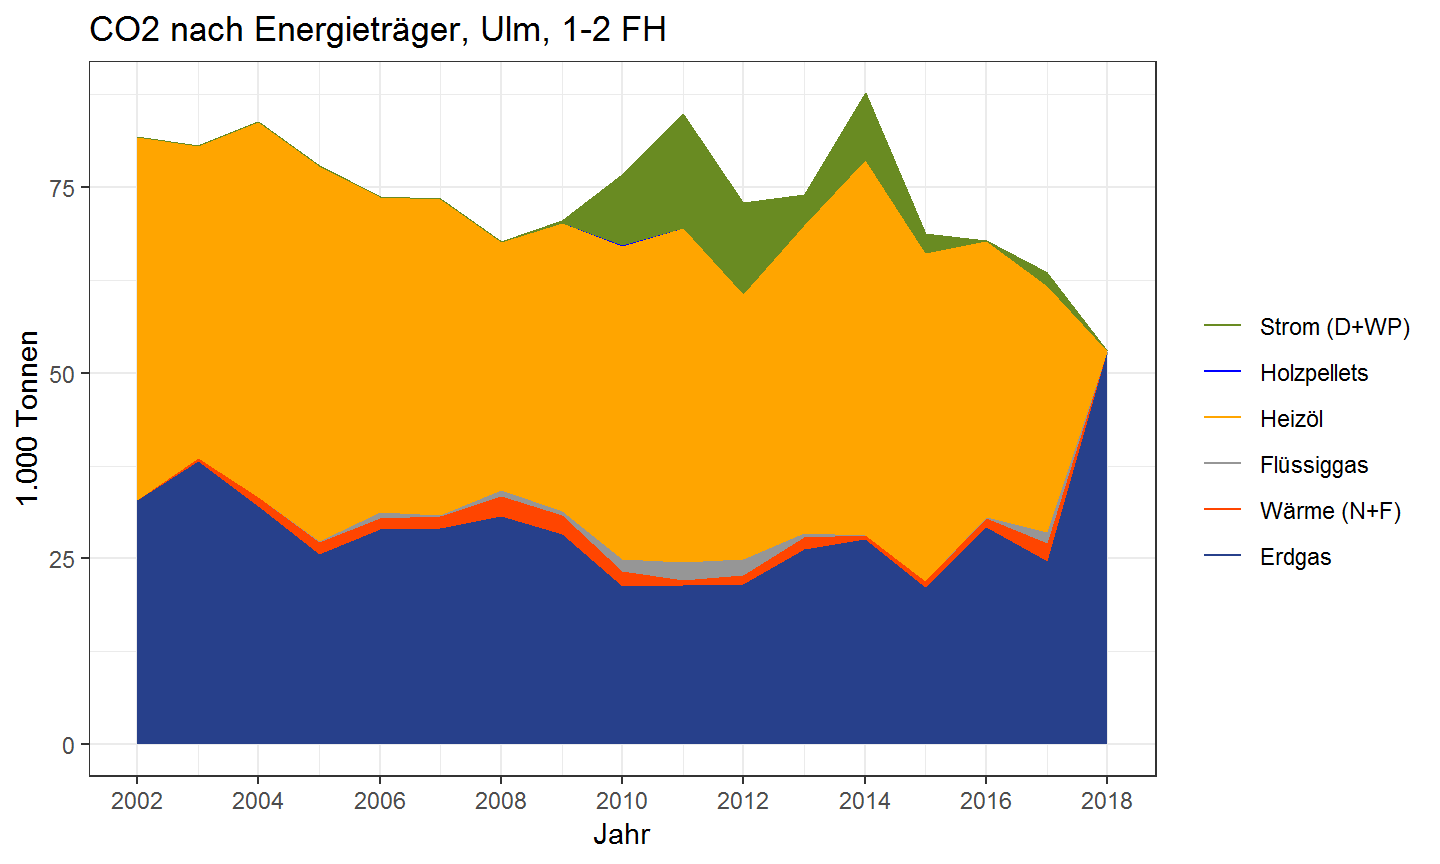
\includegraphics{UlmPresentationCO2BalanceSFH_v3_files/figure-beamer/unnamed-chunk-43-1.pdf}

\end{frame}

\begin{frame}{CO2 nach energieträger - graph}

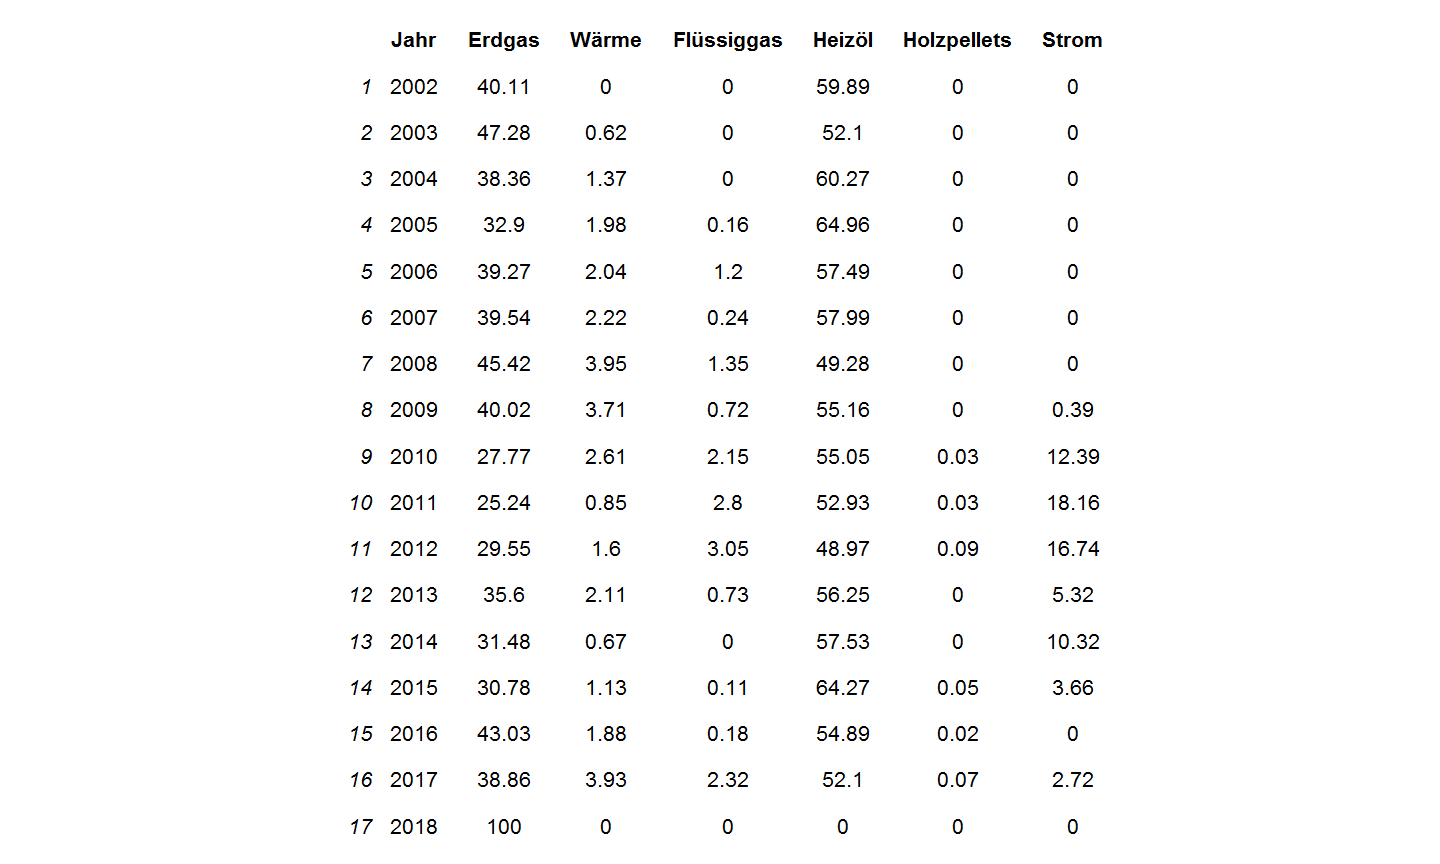
\includegraphics{UlmPresentationCO2BalanceSFH_v3_files/figure-beamer/unnamed-chunk-45-1.pdf}

\end{frame}

\begin{frame}{CO2 nach energieträger - linear graph}

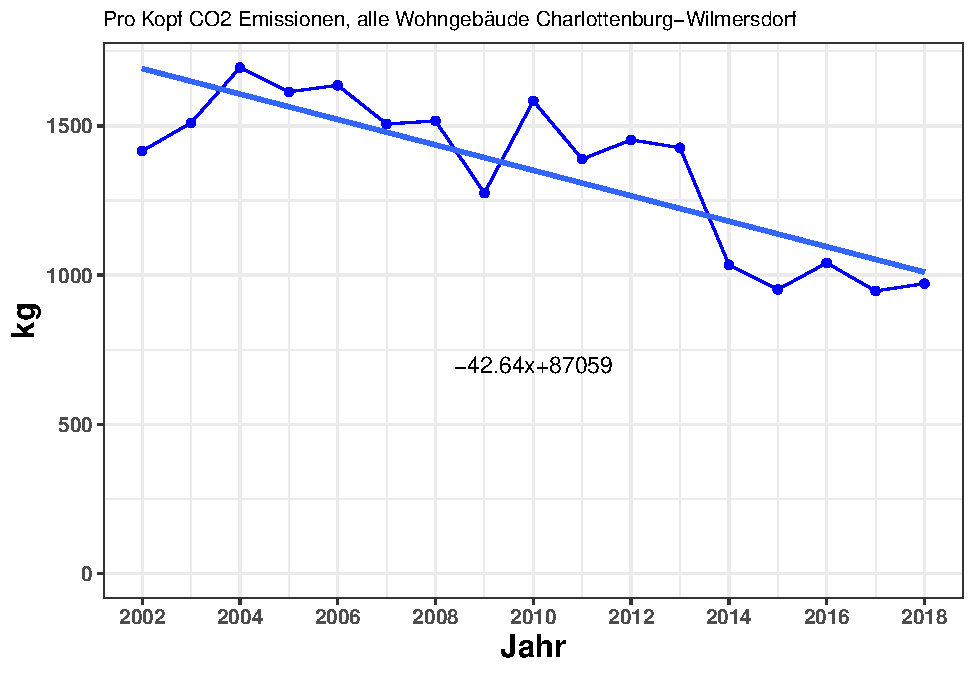
\includegraphics{UlmPresentationCO2BalanceSFH_v3_files/figure-beamer/unnamed-chunk-47-1.pdf}

\end{frame}

\begin{frame}{CO2 Anteile nach energieträger - data}

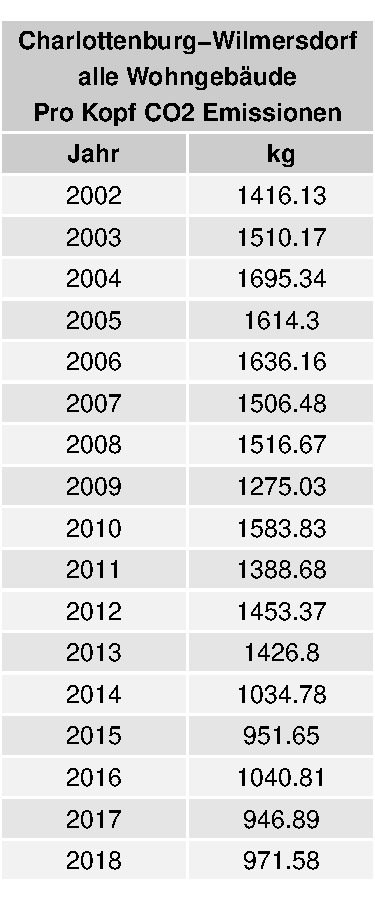
\includegraphics{UlmPresentationCO2BalanceSFH_v3_files/figure-beamer/unnamed-chunk-48-1.pdf}

\end{frame}

\begin{frame}{CO2 Anteile nach energieträger - graph}

\includegraphics{UlmPresentationCO2BalanceSFH_v3_files/figure-beamer/unnamed-chunk-50-1.pdf}

\end{frame}

\begin{frame}{CO2 Anteile nach energieträger - linear graph}

\includegraphics{UlmPresentationCO2BalanceSFH_v3_files/figure-beamer/unnamed-chunk-52-1.pdf}

\end{frame}

\begin{frame}{Spezifische CO2 Emission}

\includegraphics{UlmPresentationCO2BalanceSFH_v3_files/figure-beamer/unnamed-chunk-53-1.pdf}

\end{frame}

\end{document}
